\documentclass[a3paper,12pt]{extarticle} % Use extarticle for A3 paper size
\usepackage{graphicx} % Include this package for \includegraphics
\usepackage{amsmath}
\usepackage{amssymb} % Include this package for \mathbb
\usepackage[margin=1in]{geometry} % Adjust the margin as needed
\usepackage{algorithm} % Include this package for the algorithm environment
\usepackage{algpseudocode} % Include this package for algorithmic pseudocode

\begin{document}

\author{kipngeno koech - bkoech}
\title{Homework 5 - Introduction to Machine Learning For Engineers}   
\maketitle

\medskip

\maketitle
\section{Gaussian Mixture Models}
Consider an exponential mixture model for a 1-D dataset $\{x_n\}$ with the density function
\[
p(x) = \sum_{k=1}^K \omega_k \text{Exp}(x|\mu_k),
\]
where $K$ is the number of mixture components, $\mu_k$ is the rate parameter, and $\omega_k$ is the mixture weight corresponding to the $k$-th component. The exponential distribution is given by
\[
\text{Exp}(x|\mu) = \mu \exp(-x\mu) \quad \text{for all } x \geq 0. \tag{1}
\]

We would like to derive the model parameters $(\omega_k, \mu_k)$ for all $k$ using the EM algorithm. Consider the hidden labels $z_n \in \{1, \ldots, K\}$ and indicator variables $r_{nk}$ that are 1 if $z_n = k$ and 0 otherwise. The complete log-likelihood (assuming base $e$ for the log) is then written as
\[
\sum_n \log p(x_n, z_n) = \sum_n \sum_{z_n=k} \left[\log p(z_n = k) + \log p(x_n|z_n = k)\right].
\]

\begin{enumerate}
    \item Write down and simplify the expression for the complete log-likelihood for the exponential
    mixture model described above. Plugging the definition of the exponential distribution here immediately gives
    \[
    \sum_n \log p(x_n, z_n) = \sum_k \sum_n r_{nk} \left[\log \omega_k + \log \text{Exp}(x_n|\mu_k)\right]
    = \sum_k \sum_n r_{nk} \left[\log \omega_k + \log \mu_k - x_n \mu_k\right].
    \]
   \item  Solve the M step of the EM algorithm and find $\mu_k$ for $k = 1, \ldots, K$ that maximizes the complete log-likelihood. Taking the derivative of the log-likelihood with respect to $\mu_k$ and setting it to zero, we have:
    \[
    \frac{1}{\mu_k} \sum_n r_{nk} - \sum_n r_{nk} x_n = 0. \tag{2}
    \]
    \[
    \mu_k = \frac{\sum_n r_{nk}}{\sum_n r_{nk} x_n}. \tag{3}
    \]
    \item Perform the E step of the EM algorithm and write the equation to update the soft labels $r_{nk} = P(z_n = k|x_n)$. Using Bayes' rule, we have:
    \[
    r_{nk} = \frac{P(x_n, z_n = k)}{P(x_n)} = \frac{\omega_k \mu_k \exp(-x_n \mu_k)}{\sum_{k'} \omega_{k'} \mu_{k'} \exp(-x_n \mu_{k'})}.
    \]
\end{enumerate}

\newpage
\section{Eigen Faces}
Face recognition is an important task in computer vision and machine learning. In this question, you will
implement a classical approach called Eigenfaces. You will use face images from the Yale Face Database
B, which contains face images from 10 people under 64 lighting conditions. Please include your code in
the final PDF you turn in for full credit.

\begin{enumerate}
    \item \textbf{Dataset.} Download the data file \texttt{face\_data.mat}. It contains three sets of variables:
    \begin{itemize}
        \item \texttt{image}: each element is a face image (50 × 50 matrix). You can use \texttt{matplotlib.pyplot.imshow}
        to visualize the image. The data is stored in a cell array.
        \item \texttt{personID}: each element is the ID of the person, which takes values from 1 to 10.
        \item \texttt{subsetID}: each element is the ID of the subset which takes values from 1 to 5. Here the face
        images are divided into 5 subsets. Each subset contains face images from all people, but with
        different lighting conditions.
    \end{itemize}
    
    \item \textbf{[10 points]} Implement PCA. Fill in the function \texttt{pca\_fun} in the \texttt{pca.py} file. The function takes the
    data matrix (each row being a sample) and target dimensionality $d$ (lower than or equal to the original
    dimensionality) as the input, and outputs the selected eigenvectors.
    
    \item \textbf{[25 points]} Compute Eigenfaces. Take each 50 × 50 training image and vectorize it into a 2500-
    dimensional vector. Use your PCA implementation from part (b) to perform PCA on all vectorized
    face images, and retain the first $d = 200$ eigenvectors. These eigenvectors are called eigenfaces (when
    displayed as images). Please display the top 5 eigenfaces (use \texttt{imshow}) in your report.
\end{enumerate}

\newpage 

\section{Thompson Sampling}
Consider the Thompson Sampling (TS) algorithm, a Bayesian approach to the multi-armed bandit problem. Consider a Bernoulli bandit with $n$ arms, where each arm $i$ at time-step $1 \leq t \leq T$ has Bernoulli i.i.d. rewards $r_{i,t} \in \{0, 1\}$ with $\mathbb{E}[r_{i,t}] = \mu_i$. 

The TS algorithm starts with a prior distribution of $\mu_i$ for each arm $i$ using the $P_{i,0} \sim \text{Beta}(1, 1)$ distribution and proceeds by selecting an arm based on the posterior distribution as follows. Note the prior distribution of $\mu_i$ at time $t$ is denoted as $P_{i,t-1}$ and the posterior as $P_{i,t}$. Further, the posterior of the current time-step becomes the prior for the next time-step.

\begin{algorithm}
\caption{Thompson Sampling}
\begin{algorithmic}[1]
\For{$t = 1, 2, \ldots, T$}
    \State Sample $\hat{\mu}_{i,t} \sim P_{i,t-1}$ for each arm $i \in \{1, \ldots, n\}$
    \State Play arm $i_t = \arg \max_i \hat{\mu}_{i,t}$
    \State Observe reward $r_{i_t,t}$ and update posterior $P_{i,t}$
\EndFor
\end{algorithmic}
\end{algorithm}
Recall the probability density function of the Beta distribution, $\text{Beta}(\alpha, \beta)$, for any $x \in [0, 1]$ is
\[
p(x) = \frac{(\alpha + \beta - 1)!}{(\alpha - 1)!(\beta - 1)!} x^{\alpha - 1} (1 - x)^{\beta - 1}.
\]
We also know, for any $p, q \geq 1$,
\[
\int_0^1 x^p (1 - x)^q \, dx = \frac{(p + q + 1)!}{(p - 1)!(q - 1)!}.
\]
\begin{enumerate}
    \item \textbf{[15 points]} Until time-step $t$, suppose arm $i \in \{1, \ldots, n\}$ is pulled $N_{i,t}$ times and its total observed reward is 
    \[
    S_{i,t} := \sum_{u \leq t : i_u = i} r_{i,u},
    \]
    where $i_u$ represents the arm chosen at time-step $u$. Find $P_{i,t}$, the posterior distribution of $\mu_i$, given the Beta prior as described above and observations on the rewards until time-step $t$. 
    (Hint: Compute the posterior for the first time-step. Use this recursively for the following time-steps.)

    \item \textbf{[5 points]} Compute the mean and variance of the posterior distribution of $\mu_i$ found in part (a).

    \item \textbf{[5 points]} Using the computations in part (b), explain how TS balances exploration and exploitation.
\end{enumerate}

\newpage
\section{Gridworld}
Consider the following grid environment. Starting from any unshaded square, you can move up, down, left, or right. Actions are deterministic and always succeed (e.g., going left from state 16 goes to state 15) unless they will cause the agent to run into a wall. The thicker edges indicate walls, and attempting to move in the direction of a wall results in staying in the same square (e.g., going in any direction other than left from state 16 stays in 16).

Taking any action from the target square with cheese (no. 11) earns a reward of $r_g$ (so $r(11, a) = r_g \, \forall a$) and ends the episode. Taking any action from the square of the cat (no. 6) earns a reward of $r_r$ (so $r(6, a) = r_r \, \forall a$) and ends the episode. Otherwise, from every other square, taking any action is associated with a reward $r_s \in \{-1, 0, +1\}$ (even if the action results in the agent staying in the same square). 

Assume the discount factor $\gamma = 1$, $r_g = +10$, and $r_r = -1000$ unless otherwise specified.

\begin{figure}[H]
\centering
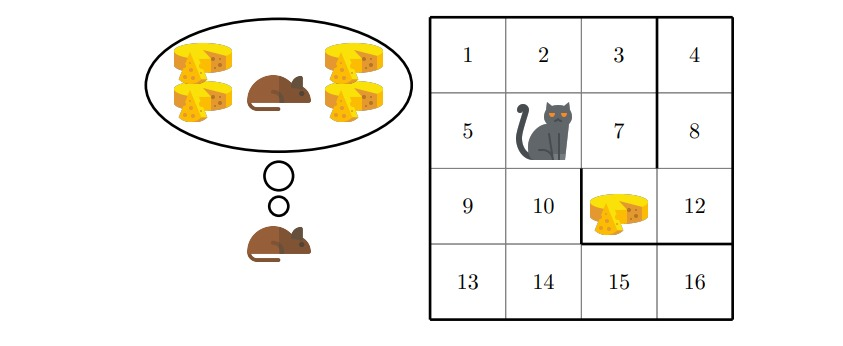
\includegraphics[width=0.8\textwidth]{grid.jpg}
\caption{Gridworld Environment}
\label{fig:gridworld}
\end{figure}

\begin{enumerate}
   \item  Let $r_s = 0$. In the policy below, the arrow in each box denotes the (deterministic) action
    that should be taken in each state. Evaluate the following policy and show the corresponding value
    (i.e., cumulative reward) for every state (square).

    \[
    \begin{array}{|c|c|c|c|}
    \hline
    \rightarrow & \rightarrow & \downarrow & \downarrow \\
    \hline
    \rightarrow & \rightarrow & \downarrow & \downarrow \\
    \hline
    \uparrow & \uparrow & \downarrow & \leftarrow \\
    \hline
    \uparrow & \uparrow & \leftarrow & \leftarrow \\
    \hline
    \end{array}
    \]
    
    \item Define the value of $r_s$ that would cause the optimal policy to return the shortest path to the
    cheese square (no. 11); note that your value for $r_s$ should lie in $\{-1, 0, +1\}$. Using this $r_s$, find the
    optimal value for each square and the optimal policy.

    \item Let’s refer to the value function derived in (b) as $V^{\pi_g}_{\text{old}}$ and the policy as $\pi_g$. Suppose we are
    now in a new gridworld where all the rewards ($r_s$, $r_g$, and $r_r$) have $+2$ added to them. Consider still
    following the policy $\pi_g$, which is optimal for the original gridworld. What will the new values $V^{\pi_g}_{\text{new}}$ be
    in this second gridworld?
\end{enumerate}

\newpage
\section{Markov Decesion Process as Linear Program}
Consider a Markov Decision Process (MDP) $M = \{S, A, P, r, \gamma\}$ where $S$ is the state space, $A$ is the action space, $P$ is the transition kernel representing the probability of transition to state $s'$ from state $s$ when action $a$ is taken as $P(s'|s, a)$, $r$ is the reward function, and $\gamma$ is the discount factor. Consider the linear program:
\[
\min_{V \in \mathbb{R}^{|S|}} \sum_{s \in S} \rho(s)V(s)
\]
subject to
\[
V(s) \geq r(s, a) + \gamma \sum_{s' \in S} P(s'|s, a)V(s') \quad \forall s \in S, \, a \in A,
\]
where $\rho(s) \in \mathbb{R}_+ \, \forall s \in S$ and denote its solution as $V^\star \in \mathbb{R}^{|S|}$.

\begin{enumerate}
    \item Show that the dual formulation of the above linear program can be written as
    \[
    \max_{x \in \mathbb{R}^{|S| \times |A|}} \sum_{s \in S} \sum_{a \in A} r(s, a)x(s, a)
    \]
    subject to
    \[
    \sum_{a \in A} x(s, a) - \gamma \sum_{s' \in S} \sum_{a' \in A} P(s|s', a')x(s', a') = \rho(s) \quad \forall s \in S,
    \]
    \[
    x(s, a) \geq 0 \quad \forall s \in S, \, a \in A.
    \]
   \item Denote the optimal solution to the dual problem as $x^\star \in \mathbb{R}^{|S \times A|}$. Due to strong duality
    and complementary slackness, we have
    \[
    x^\star(s, a) \left(V^\star(s) - \gamma \sum_{s' \in S} P(s'|s, a)V^\star(s') - r(s, a)\right) = 0 \quad \forall s \in S, \, a \in A.
    \]
    Now, show that the optimal policy $\pi^\star(\cdot|s), \, \forall s \in S$, can be derived as
    \[
    \pi^\star(a|s) =
    \begin{cases}
    1 & \text{if } a = \arg \max_{a \in A} x^\star(s, a), \\
    0 & \text{else}.
    \end{cases}
    \]
\end{enumerate}

\end{document}